
\section{Application Payloads}

While the amount of computation done in a single speculative execution is small,
we demonstrate several applications that can take advantage of multiple
speculative runs to carry out computation.

As a first step, we observe that this primitive can be used to trivially
implement a finite state machine: any logic can be done in the speculative
world, while
updates to the state are communicated to the real world where they are stored.
On the next run of the speculative instructions, they read from the real world
state (and other inputs), compute any state transitions, and communicate the
result. In this mode, the state is maintained by the real world, while updates
are controlled by code executed speculatively.

\begin{figure}[t]
    \centering
        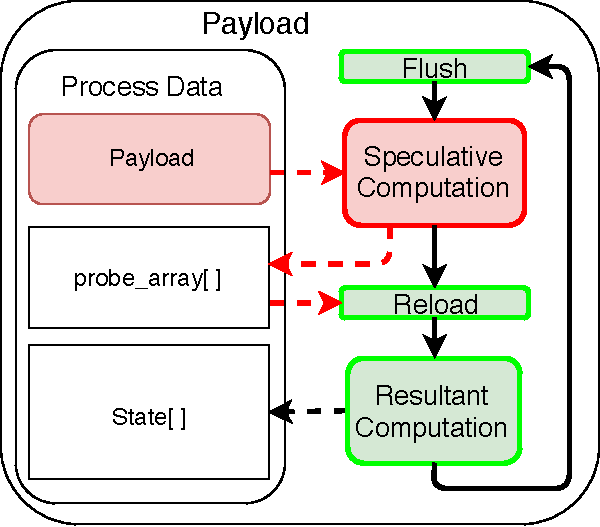
\includegraphics[width=0.4\textwidth]{figures/general_model}
    \caption{ General model of speculative computation within the Measure 
        process when triggered. \textit{Speculative Computation} has access
        to all variables which do not require a memory transaction within
        the current state of the process. The process can subsequently make
        \textit{Resultant Computations} based on the value returned from 
        Prime and Probe to update the state of the process. }
    \label{fig:general_model}
\end{figure}


\subsection{Turing Machine}
\label{subsec:turing}
- Arbitrary computation

\subsection{Unpacking and Decryption}
\label{subsec:decryption}
While Section \ref{subsec:turing} demonstrates that arbitary computation is
possible, if a reverse engineer can discover the \emph{speculative instructions}
they can determine the execution of this program by simply reading the
instructions that are passed along. To avoid this we can encrypt the
\emph{speculative instructions}, meaning that a reverse engineer can never
determine these instructions by examining the ELF file, or generating source
code. 

The encrypted code must be decrypted so that the instructions can be executed.
In order to obscure this information from the ``real world'' the speculative
world must do the decryption. As such we have built a prototype capable of
decrypting messages in the speculative world and passing the results back to the
real world in pieces.

The speculative world is able to take advantage of the AES-NI instructions to
decrypt messages. In order to avoid detection (as well as reduce the computation
that needs to be done in the speculative world) the key expansion can be done
ahead of time. However, the key schedule does have a structure that could be
detected by a reverse engineer. Thus 11 random round keys are selected. This
obfuscated key schedule makes it more difficult for a reverse engineer to
determine that there is encrypted content. Additionally since the content is
only accessed when the correct trigger program is running the challenges facing
a reverse engineer are great.


% 
% Argument for obfuscating keyschedule
% 
% Challenge for Rev-Engineer
%   - Find the obfuscated key schedule
%   - Find the correct trigger program

\subsection{Virtual Machines}
Given the specific constraints that the speculative environment enforces on
these paylods, general purpose compuatation []. We demonstrated in
section~\ref{subsec:turing} that general purpose computation is possible using
computation performed in the speculative environment. However, a turing machine
is not a user friendly model, nor is it an efficient model for computation when
attempting to accomplish tasks on modern processors. 

Using emulators in the "real world" allows for crafted binary programs to be 
instrumented in dead code and, as demonstrated in secton~\ref{subsec:decryption} 
encrypted and hidden. This gives an advantage to attackers as traditional 
reverse engineering methods will reveal only that emulation is being done. 
It reveals nothing about the ultimate goal of the program. 

To accomodate both developers as well as the unique constraints 
enforced by the speculative primitive, a custom emulation solution is required. We 
have approached this challenge from both directions. First we demonstrate 
general purpose emulation using a custom instruction set -- SPASM -- which
accomodates the speculative primitive specifically. Next we investigate custom 
wrappers on traditional emulators allow for similar payload construction,
with a much more developer friendly 

% REFERENCE FIGURES
% - Constraints enforced by speculative primitive
%       - more bits = slower
%       - less bits = less expressive
%       - must be computable within speculative ROB limit (~150 instrs) (decrypt only)
%   
% - optimizations for weird-machine computations 

% --- VM
%   - Wrappers around traditional ISA VMs
%   - SPASM  custom emulator made f
%%%%%%%%%%%%%%
